\chapter{Introduction}\label{ch:introduction}

\vspace{0.5cm} 

"An individual economic variable, views as a time series, can wander extensively
and yet some pairs of series may be expected to move so that they do not drift
far apart."-Robert F. Engle and Clive W.J. Granger~\cite{engle1987}.\\
In this introduction we present the scope, objectives, hypothesis and organization of this thesis.


\section{Introduction}
A time series is a sequence S of historical measurements y t of an observable
variable y at equal time intervals. Time series are studied for several purposes
such as the forecasting of the future based on knowledge of the past, the un-
derstanding of the phenomenon underlying the measures, or simply a succinct
description of the salient features of the series. In this chapter we shall
confine
ourselves to the problem of forecasting. Forecasting future values of an
observed
time series plays an important role in nearly all fields of science and
engineering,
such as economics, finance, business intelligence, meteorology and telecommu-
nication [43]. An important aspect of the forecasting task is represented by the
size of the horizon. If the one-step forecasting of a time series is already a
chal-
lenging task, performing multi-step forecasting is more difficult [53] because
of

additional complications, like accumulation of errors, reduced accuracy, and in-
creased uncertainty [58,49].
The forecasting domain has been influenced, for a long time, by linear sta-
tistical methods such as ARIMA models. However, in the late 1970s and early
1980s, it became increasingly clear that linear models are not adapted to many
real applications [25]. In the same period, several useful nonlinear time series
models were proposed such as the bilinear model [44], the threshold autoregres-
sive model [56,54,55] and the autoregressive conditional heteroscedastic (ARCH)
model [22] (see [25] and [26] for a review). However, the analytical study of
non-
linear time series analysis and forecasting is still in its infancy compared to
linear
time series [25].
In the last two decades, machine learning models have drawn attention and
have established themselves as serious contenders to classical statistical
models
in the forecasting community [1,43,61]. These models, also called black-box or
data-driven models [40], are examples of nonparametric nonlinear models which
use only historical data to learn the stochastic dependency between the past and
the future. For instance, Werbos found that Artificial Neural Networks (ANNs)
outperform the classical statistical methods such as linear regression and Box-
Jenkins approaches [59,60]. A similar study has been conducted by Lapedes and
Farber [33] who conclude that ANNs can be successfully used for modeling and
forecasting nonlinear time series. Later, other models appeared such as decision
trees, support vector machines and nearest neighbor regression [29,3]. Moreover,
the empirical accuracy of several machine learning models has been explored in a
number of forecasting competitions under different data conditions (e.g. the
NN3,
NN5, and the annual ESTSP competitions [19,20,34,35]) creating interesting
scientific debates in the area of data mining and forecasting [28,45,21].


%%%%%%%%%%%%%%%%%%%%%%%%%%%%%%

The computational complexity of machine learning algorithms has become a limiting factor for problems that require processing large volumes of data and where the response time is crucial. An example of this is financial volatility time series forecast. 

Currently, it is known that volatility is a process where many factors influence its behaviour. However, many models of volatility made forecasts based only on price returns. Examples are the ARFIMA, GARCH and stochastic volatility models. Machines learning methods have allowed a greater number of explanatory variables to be included, although in many cases, these increase calculation time. 

Algorithms that process large amounts of data in a short time and are able to detect changes in the financial market are required to achieve fast and accurate responses. Online learning algorithms have been developed to solve large-scale problems since they process an instance at a time, updating the model at each step incrementally. This is opposed to the batch algorithms where a phase of training that uses a large collection of historical data is first required and the resulting model is later used to predict. 
This thesis proposal is to design and develop an online learning algorithm that meets or improves the performance of current volatility algorithms and ensures rapid responses to large-scale problems. Model comparisons will be made by the SPA (superior predictive ability) test proposed by Hansen and
Lunde~\cite{hansen+lunde2006}  that allows comparing of forecast models giving a relative measure of model performance with respect to one or more models.



\section{The problem}

In financial markets, volatility is one of the key elements to model the stochastic dynamic behaviour of financial assets. This is mainly because volatility gives a measure of uncertainty about future returns and it is often viewed as an indicator of the vulnerability of financial markets. It is also important as an input parameter in problems like derivative pricing, hedging and portfolio management. For example, in option pricing we need to known first the volatility of the underlying asset before pricing an option. 

Besides, volatility provides important information for studying asset returns because the latter are largely uncorrelated and nonlinearly dependent. However, it has been found that volatility exhibits significant autocorrelation and predictable patterns~\cite{poon+granger2003} and  many models have been proposed to forecast its behaviour (see section ~\ref{sec:stylizedfacts}).

The volatility of the data is due to a large number of factors affecting the market, with some of them directly measurable such as historical prices, trends, supply and demand. However, others such as monetary policies and news are not directly measurable and are included in other models out of the scope of this thesis. Figure~\ref{fig:VolFactorNews} shows the VIX index, the daily US implied stock market volatility, commonly known as the "financial fear factor" which is clearly affected by historical events.


\begin{figure}[h]
 \centering
 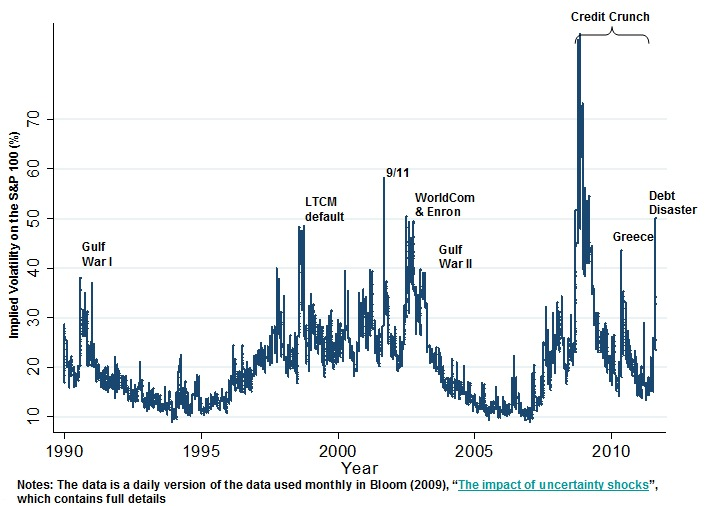
\includegraphics[width=0.7\textwidth]{img/vol-factor-thenews.jpg}
 % vol-factor-thenews.jpg: 710x506 pixel, 72dpi, 25.05x17.85 cm, bb=0 0 710 506
 \caption{The news as volatility factor}
 \label{fig:VolFactorNews}
\end{figure}


Volatility models have been extensively studied~\cite{gatheral2006,poon+granger2003,knight2002} and some of  them include machine learning methods~\cite{hamidetal2004,donaldsonetal1997,shiyietal2008,shiyietal2010,gavrishchaka2006,vasilios2012}.  
The stochastic behaviour of volatility and the large number of factors affecting it result in models with a large number of parameters and slow response time due to the computationally expensive routines. These expensive calculations could be avoided using online learning algorithms, which allow response time reduction and are therefore suitable for high frequency trading applications. 

In this thesis, a model will be proposed based on online learning algorithms to forecast volatility in high frequency financial time series.
The main problems to be deal with in this thesis are:

\begin{itemize}
   \item Although volatility is often predictable~\cite{poon+granger2003}, there are non-linear features~\cite{gatheral2006} to be considered in this proposal.
    \item The number of factors affecting volatility has been studied~\cite{srinivasan2009} and some other unknown factors affect volatility and they should also be included.
    \item The response time needs to be very fast and in order to ensure this, the proposed model will be presented as an online machine learning algorithm. 
\end{itemize}





\section{Scope of this Research}

Cointegration concept was introduced by~\cite{engle1987} and implies that one or
more linear combinations of non-stationary variables are stationary even though
individually they are not.  Moreover ~\cite{stock+watson1988} observed that
cointegration reflects the common stochastic trends providing a useful way to
understand cointegration relationships. These common stochastic trends can be
also interpreted as a long-run equilibrium relationships.

This idea was inmediatly adopted in finance since it could represent their
long-run relationship implied by economic theory~\cite{laietAl1991},
\cite{lence+falk2005}.  Economic theory suggest that economic time series are
mean-reverting process and therefore, it reflects the idea of that some set of
variables cannot wander too far from each other. 

On the other hand, the efficient markets hypothesis, also known as the random
walk theory states that current stock prices fully reflect available
information related to its value and there is no way to earn excess
profits~\cite{fama1970}.  This means that if we have stock prices from a
jointly efficient market, they cannot be
cointegrated~\cite{granger1986},\cite{dwyer1992}. However, \cite{richards1995}
claims that cointegration is directly at odds with market efficiency, even
though, there is no evidende that cointegration among asset prices have
implications about market efficiency~\cite{lence+falk2005}.

Despite the fact that cointegration on closing daily rates of currency pairs has
not been found \cite{coleman1990}, \cite{copeland1991}, different time series
frequencies can have different behaviours~\cite{aldridge2009}. Pair trading is a
very common example of cointegration application~\cite{herlemont2003} 
but cointegration can also be extended to a larger set of
variables~\cite{mukherjee1995},\cite{engle2004}.

%So why do we care about cointegration? Someone else can probably give more
%econometric applications, but in quantitative finance, cointegration forms the
%basis of the pairs trading strategy: suppose we have two cointegrated stocks X
%and Y, with the particular (for concreteness) cointegrating relationship X - 2Y
%= Z, where Z is a stationary series of zero mean. For example, X could be
%McDonald's, Y could be Burger King, and the cointegration relationship would
%mean that X tends to be priced twice as high as Y, so that when X is more than
%twice the price of Y, we expect X to move down or Y to move up in the near
%future (and analogously, if X is less than twice the price of Y, we expect X to
%move up or Y to move down). This suggests the following trading strategy: if X -
%2Y > d, for some positive threshold d, then we should sell X and buy Y (since we
%expect X to decrease in price and Y to increase), and similarly, if X - 2Y < -d,
%then we should buy X and sell Y.


Vector error correction model (VECM) introduces this long-run relationship
among a set of cointegrated variables as an error correction term. VECM is a
special case of the vector autorregresive model (VAR) model. VAR model
expresses future values as a linear combination of variables past values.
However, VAR model cannot be used with non-stationary variables. VECM is a
linear model but in terms of variable differences. If cointegration exists,
variable differences are stationary and they introduce an error correction term
which adjusts coefficients to bring the variables back to equilibrium. In
finance, many economic time series turn to be stationary when they are
differentiated and cointegration restrictions often improves
forecasting~\cite{duy1998}. Therefore, VECM has been widely adopted.

Both VECM and VAR model parameters are obtained using ordinary least squares
(OLS) method. OLS has two main problems: is sensitive to errors on input data
and involves many calculations. The former problem is commonly solved using
Ridge Regression (RR) \cite{hoerl1970} which introduces a regularization
parameter that leads to an unbiased estimation with better generalization
capability. The second problem of computational complexity depends on the number
of past values and observations considered.  Recently, online learning
algorithms have been proposed to solve problems with large data sets because of
their simplicity and their ability to update the model when new data is
available. 

In this thesis, we propose an online formulation of the VECM called Onlive VECM
(OVECM) based on consideration of only a sliding window of the most recent data.
The algorithm introduces matrix optimizations in order to reduce the number of
operations and also takes into account the fact that cointegration vector space
doesn't experience large changes with small changes in the input data. Moreover,
RR instead of OLS is used to solve VECM. Our method is later tested using four
currency rates from the foreign exchange market with different frequencies.  Model
efectiveness is focused on out-of-sample forecast rather than in-sample fitting.
This criteria allows the OVECM prediction capability to be expressed rather than
just explaining data history. Our method performance is compared with its
optimal offline algorithm.


\section{Research Objectives}
The main motivation for this research is ...

The specific objectives of this research are,
\begin{itemize}
\item $\Large \mathcal{O}_1$: \emph{Especific Objective 1.}
\item $\Large \mathcal{O}_2$: \emph{Especific Objective 2.}
\item $\Large \mathcal{O}_3$: \emph{Especific Objective 3.}
\item $\Large \mathcal{O}_4$: \emph{Especific Objective 4.}
\item $\Large \mathcal{O}_5$: \emph{Especific Objective 5.}
\end{itemize}


\section{Research Hypothesis}


The main research hypothesis explored in this dissertation is the following \\

\textit{Hypothesis llll . }

\section{Organization of this Thesis}

Chapter 1 contains ...





%\section{Hypotheses}
%
%
%Volatility forecasting has been a largely studied and different approaches have arisen to describe its stochastic behaviour. It is well-known that volatility depends on many factors, but most of the existing models only consider a few of them. In order to introduce more factors easily, classic machine learning models have been studied and their performance have shown to be successfull in comparison with most used volatility models. However, their training process is computationally expensive and it is not possible to update the model with new market information before new information arrives. Online learning methods can also include more factors into a model, but they process one example at a time to update an existing model incrementally without having a training phase, thus they improve response times and are more suitable for financial applications.
%
%
%The thesis hypotheses are the following:
%
%\begin{enumerate} 
%\item Machine learning based models that consider more volatility explanatory factors will adapt and perform better than popular volatility forecasting models based only on returns or a few factors.
%\item Stylized facts can be efficiently introduced as explanatory factors and improve model performance.
%\item The use of online learning methods will allow inclusion of as many variables as needed to ensure low response times.  
%\end{enumerate}
%
%\section{General Objective}
%To design and implement an online learning model for volatility forecasting capable of adapting to their non-stationary behaviour using volatility factors as model input ensuring low response times.  
%\section{Specific Objectives}
%The specific objectives to be followed in this thesis are:
%\begin{enumerate}
%  \item To determine the best volatility factors based on their stylized facts and their performance in machine learning models.
%  \item To determine the best sampling of high frequency time series.
%  \item To define the best realized volatility proxy based on the literature and experimental results.
%  \item To design and implement a novel online learning algorithm with large input factors capable of ensuring low response time.
%  \item To modify the original algorithm using kernel trick and evaluate its performance.
%  \item To compare performance of the most popular algorithms for volatility forecasting such as ARFIMA, GARCH and SV models.
%  \item To assess the predictive capacity of the proposed model using the SPA test.
%  \item To compare the performance of the most popular models and the proposed model using real financial data.
%\end{enumerate}


%\section{Thesis proposal}
%
%This thesis proposal is to build an algorithm to forecast realized volatility in financial markets considering not only intraday returns but also other explanatory volatility variables. Because of the amount of high frequency data to be considered and short response times required in financial applications, the algorithm will be formulated in online mode. The online algorithm will also allow the shifting problem to be tackled while being adaptive to wild changes in the volatility process.
%The online learning model will be formulated considering the following:
%
%\begin{description}%[leftmargin=0.4cm]\itemsep4pt
%    \item[large volumes of data:] high frequency data will be used to estimate realized volatility. The frequency to be considered will be 10 to 15 minutes. This frequency will be analysed using signal processing theory. 
%    \item[non-stationary data:] volatility is a time series known because of its non-stationary feature, so statistics will be studied before using the model.
%    \item[stylized facts:] there are several well-documented features about financial time series volatility called stylized facts~\cite{poon+granger2003} that can be included in the model.
%    \item[low response time:] the model has to be simple but powerful in order to achieve the response time needed. If the model is extended to real time data, ticks can arrive at rates of milliseconds and the model should respond at the same rate or less.
%    \item[financial data:] the model can be constructed using data of stocks or different derivatives such as options and futures. The chosen implicit volatility model will depend on the data type.
%    \item[input vector:] currently, many models are only based on expected returns, but volatility is a complex variable which depends also on many factors studied in the literature such as trading volume, the tick rate, time of the day and the behaviour of the market as a hole~\cite{gatheral2006}. All these factors can improve the design of the proposed online algorithm.
%    \item[kernel version:] the online algorithm will be later kernelised in order to map the input data into a high dimensional feature space (kernel trick) which will provide better properties to design the solution.
%\end{description}
%
%The model proposed has to be compared with the current popular financial models of financial volatility such as: ARFIMA, GARCH, SV models and machine learning models. Performance will be measured using the realized volatility shown in equation~(\ref{eq:srv}) as a benchmark.
%
%In order to compare different models, apart from using the standard performance measurements like MAE and MSE, the superior predictive ability (SPA) methodology proposed by Hansen and Lunde~\cite{hansen+lunde2006} will also be studied. SPA is a test to compare two or more forecasting models at the same time giving a relative performance measurement of a base model in comparison with alternative models. 
%
%The model will be compared against traditional financial volatility models such as Black-Scholes, SV, GARCH and ARFIMA using different forecast errors measurements. Although the best way to measure forecast errors should be the investor returns, this implies knowing how the model information is used as a strategy, so this information is not going to be included in this thesis. Therefore, in order to compare the different volatility forecast models, popular evaluation measurements will be used. In the literature the following are commonly used: {\em Mean Error} (ME), {\em Mean Square Error} (MSE), {\em Mean Absolute Error} (MAE) and {\em Mean Absolute Percent Error} {MAPE} and others are less commonly used such as LINEX loss function which weight differently positive and negative errors. In ~\cite{granger1999} Granger describes a variety of non-symmetric loss function including LINEX. The superior predictive ability (SPA) methodology proposed by Hansen and Lunde~\cite{hansen+lunde2006} will also be studied 
%which allows comparison of two or more forecasting models at the same time giving a relative performance measurement of a base model compared with alternative models.  All these measurements will be out-of-sample in order to show their predictive power.
